\chapter{Media Item Compilation}
\label{cha:media-item-compilation}

% the code below specifies where the figures are stored
\ifpdf
    \graphicspath{{9_media_item_compilation/figures/PNG/}{9_media_item_compilation/figures/PDF/}{9_media_item_compilation/figures/}}
\else
    \graphicspath{{9_media_item_compilation/figures/EPS/}{9_media_item_compilation/figures/}}
\fi

\section{Introduction}

In this chapter, we introduce aesthetic principles
for the automated generation of media galleries
based on media items retrieved from social networks
that---after a~ranking and pruning step---can serve to authentically
summarize events and their atmosphere from a~visual
and an audial standpoint.
Mobile devices such as smartphones, together with social networks,
enable people to create, share, and consume media items
like videos or photos.
These devices accompany their owners almost everywhere
and are thus omnipresent at all sorts of events.
At such events---given a~stable network connection---part of
the event-related media items are published on social networks
both as the event happens or afterwards,
once a~stable network connection has been established again.
Ranked media items stemming from multiple social networks
can serve to create authentic media galleries
that illustrate events and their atmosphere.
A~key feature for this task is the semantic enrichment
of media items and associated microposts
and the extraction of \emph{visual}, \emph{audial},
\emph{textual}, and \emph{social} features.
Based on this set of features,
additional \emph{aesthetic} features
can be defined and exploited to obtain appealing
and harmonic media galleries.

\section{Related Work}

While enormous efforts have been made to extract
\emph{visual}, \emph{audial},
\emph{textual}, and \emph{social} features
from media items and microposts on social networks in \emph{isolation},
to the best of our knowledge, remarkably less initiatives 
concern the extraction and the application
of all those features \emph{in combination}
for \emph{all} types of media items, including microposts.
In~\cite{sandhaus2011photobook}, Sandhaus \emph{et~al.}\ consider visual and
aesthetic features for the automated creation of photo books.
Obrador \emph{et~al.}\ use visual and aesthetic features
for a~category-based approach to automatically assess
the aesthetic appeal of photographs~\cite{obrador2012photoaesthetics}.
In~\cite{knees2006musicplaylist}, Knees \emph{et~al.}\ use audial and textual
features for the automatic generation of music playlists.
Choudhury \emph{et~al.}\ show in~\cite{choudhury2011sportstweets} how social and textual
features can be used to achieve precise detection results 
of named entities and significant events in sports-related microposts.
In~\cite{davidson2010videorecommendation}, Davidson \emph{et~al.}\ show how visual,
textual, and social features can be used for personalized video recommendations.
A service called Storify~\cite{fincham2011storify} lets users manually combine
microposts, photos, videos, and other elements onto one page for the purpose
of storytelling or summarizing an event
and share stories permanently on the Web.
Finally, social networks present photos and videos
often in grid-like galleries,\footnote{\url{http://twitpic.com/904yka/full}, accessed July 15, 2013}
sometimes scaled based on the amount of comments.
When unique media items have been collected,
the remaining task is to summarize events by selecting the most relevant media items or media fragments. 
Fabro and B\"osz\"orm\'enyi~\cite{delfabro2012summarization} detail
the summarization and presentation of events from content retrieved from social media.
Nowadays, many domain-specific methods already exhibit good accuracy,
for example, in the sports domain~\cite{li2001sportsvideo,li2010americanfootball}. However, the challenge is to find methods that are content-agnostic.
Methods that exploit semantic information~(\emph{e.g.},~\cite{chen2009videosummarization}) 
will likely provide high-quality results in the future,
but today's most relevant summaries are produced by user interaction~\cite{olsen2011videosummarization}.

\section{Media Gallery Aesthetics}

\paragraph{Definition:}

A media gallery is a~compilation of photos or videos
retrieved from social networks that are related to a~given event.
Given a~set $M_{start} = \{m_1,..., m_n\}$ of media items related to a~certain event,
a~ranking formula $f$, and a~ranking threshold $t$,
the resulting subset $M_{final} \subset M_{start}$
is the result after the application of $f$ to $M_{start}$: $f(M_{start})=M_{ranked}$
and pruning the ranked set $M_{ranked}$ to only include members
whose rank is greater than $t$, with the resulting set named $M_{final}$.
Each media item $m_i$ can either be an instance of video or photo.
For each point $t_x$ on a~timeline $T$, the state of the media gallery
at $t_x$ is defined for each media item $m_i$
as a~set $S_x$ of $n$ tuples $s_{x,i}$, where
$s_{x,i}=\langle \mathit{left}$, $\mathit{top}$, $\mathit{width}$, $\mathit{height}$,
$\mathit{alpha}$, $\mathit{z\mbox{-}index}$, $\mathit{animation}$,
$\mathit{start}$, $\mathit{playing}$, $\mathit{volume} \rangle$.
The first six properties are defined as in CSS~%
\cite{bos2011css}, the $\mathit{animation}$ property
allows for the definition of CSS transitions as defined in~%
\cite{jackson2013csstransitions}
and CSS transformations as defined in~%
\cite{fraser2012csstransforms},
the $\mathit{start}$ property defines the start time in a~video.
The property $\mathit{playing}$ describes whether a~video is currently paused or playing.
Finally, the property $\mathit{volume}$ describes the volume level
of a~video.
A schematic media gallery at $t_x$ can be seen in \autoref{fig:media-gallery}.

\begin{figure}[!ht]
  \centering
  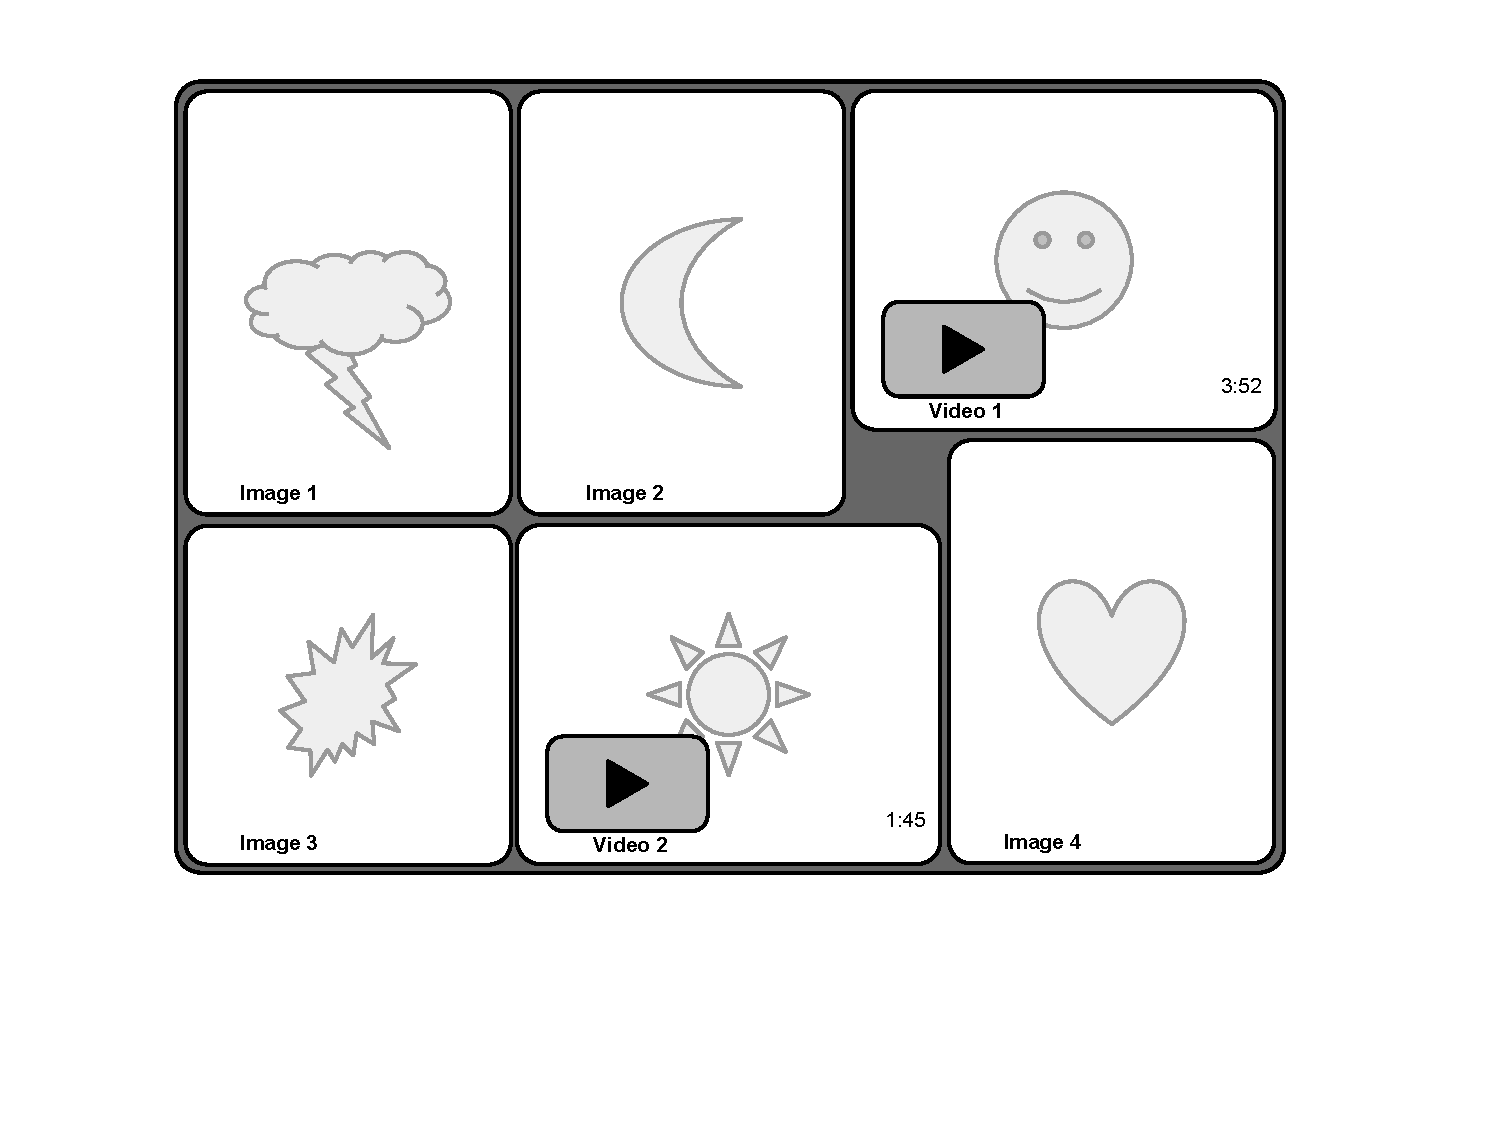
\includegraphics[trim=20mm 40mm 20mm 10mm, clip, width=0.7\columnwidth]{media-gallery.pdf}
  \caption{Schematic media gallery with four photos and two videos}
  \label{fig:media-gallery}
\end{figure}

\paragraph{Audial aesthetics:}

We recall the purpose of our media galleries:
to illustrate an event and its atmosphere.
Audial aesthetics thus consist of aspects like volume level normalization,
avoiding multiple videos playing music in parallel, smooth transitions, \emph{etc.}
We remark that through selective mixing of audio tracks
of event-related videos, ``noise clouds''
that are very characteristic
for an event's atmosphere can be observed.
We support this by allowing users to play more than one video at a~time.

\paragraph{Visual aesthetics:}

Visual aesthetics are determined by the composition, \emph{i.e.},
the relation of the number of photos \emph{vs.} the number of videos \emph{globally},
\emph{per coherent scene}, and per \emph{point in time}.
In order to avoid cognitive overload of viewers,
the number of visible (moving) media items
at a~time should be limited.
We will treat this topic in more detail in \autoref{sec:user-studies}.
Depending on the event, a~consistent or a~contrast-rich overall
appearance of items may be desired,
this also applies to transitions.

\section{Motivation for Automated Media Gallery Generation}
\label{sec:motivation-chapter-8}

Media galleries (see \autoref{fig:media-gallery1} and \autoref{fig:media-gallery2}
for examples)
help users consume significant
amounts of media items in an ideally pleasing and aesthetic way.
These media items may---or, more commonly: may not---be ordered,
besides an intrinsic chronologic order.
In the context of our work on summarizing events
based on microposts and media items stemming from
multiple social networks, we have created methods
to first \emph{extract} event-related media items
from multiple social networks, second, to
\emph{deduplicate} near- and exact-duplicate media items,
third, to \emph{cluster} them by visual similarity, and
finally, to \emph{rank} the resulting media item clusters
according to well-defined ranking criteria.
In this chapter, we treat the challenge of \emph{compiling}
ranked media item clusters in media galleries in ways
such that the ranking-implied order is at least loosely respected.
In the previous section, we have defined
aesthetic principles for automated media gallery layout~\cite{steiner2012definingaesthetic},
which we now apply to media gallery styles.
The task of media gallery compilation is different
from the widely researched task of photo book generation,
as media galleries can contain both photos and videos.
Different types of media gallery layouts are possible,
two of which we have implemented and evaluated via two different user studies:
one with, and one without detailed user comments.

\section{Media Gallery Styles}
\label{sec:mediagallerystyles}

Media galleries---in contrast to free-form digital media collages---%
necessarily display media items in a~grid-like way.
The crucial question is thus whether the media items' aspect ratios
should be respected, or whether they should be cropped to square,
or other aspect ratios (\emph{e.g.}, 4:3 or 16:9).
Respecting the aspect ratio has the advantage that media items
do not need to be cropped, which may affect important contained information like, \emph{e.g.}, 
contained faces or text.
However, due to the unpredictable media item formats,
compiling media galleries that do not look frayed is harder.
The advantage of cropping is that media gallery layout is easier,
as the media item formats are predictably the same,
at the cost of having to decide where to crop.
Different algorithms (\emph{e.g.},~\cite{suh2003thumbnail})
beyond this chapter's scope exist to aid this decision.

We use the following terminology.
A~media gallery is called \emph{balanced} if its shape is rectangular,
\emph{hole-free} if there are no gaps from missing media items,
and \emph{order-respecting}
if media items appear in insertion order.
Optimal media galleries fulfill all three conditions.

\paragraph{Non-Order-Respecting Styles:}

An interesting technique for arranging media items is dividing.
Paper sizes that follow the ISO~216 standard%
\footnote{\url{http://www.iso.org/iso/iso_catalogue/catalogue_tc/catalogue_detail.htm?csnumber=36631},
accessed July 15, 2013}
are the most common every-day examples of the dividing principle:
every media item with an aspect ratio of $ \sqrt2 $ can be divided
into two media items with the same aspect ratio%
~\cite{chedeau2012lightboxandroid}.
This works for portrait and landscape orientations,
however, is not necessarily order-respecting.
Two other non-order-respecting techniques are (i)~%
working with pre-defined placeholder patterns
(small and big squares, portrait and landscape rectangles)
and then filling the placeholder shapes with media items%
~\cite{chedeau2012500px}
or (ii)~working with columns of pre-defined widths
and then iteratively inserting in the smallest column%
~\cite{chedeau2012lightbox}.

As outlined in \autoref{sec:motivation-chapter-8},
we require (at least loosely) order-respecting media galleries
for the ranking step to make sense.
In the upcoming two paragraphs, we will introduce two techniques
for the generation of such media galleries.

\paragraph{Strict Order, Equal Size (SOES):}

A~media gallery style that we call \emph{Strict Order, Equal Size (SOES)},
which strictly respects the ranking-implied order is presented in~%
\cite{chedeau2012googleplus}.
Examples can be seen in \autoref{fig:a} and \autoref{fig:c}.
The algorithm works by resizing all media items in a~row to the same height
and adjusting the widths in a~way that the aspect ratios are maintained.
A~row is filled until a~maximum row height is reached,
then a~new row (with potentially different height) starts, \emph{etc.}
This media gallery style is strictly order-respecting, hole-free,
and can be balanced by adjusting the number
of media items in $+1$ steps.

\begin{figure}[!ht]
  \centering
  \subfloat[\emph{SOES}, Survey~A]{
    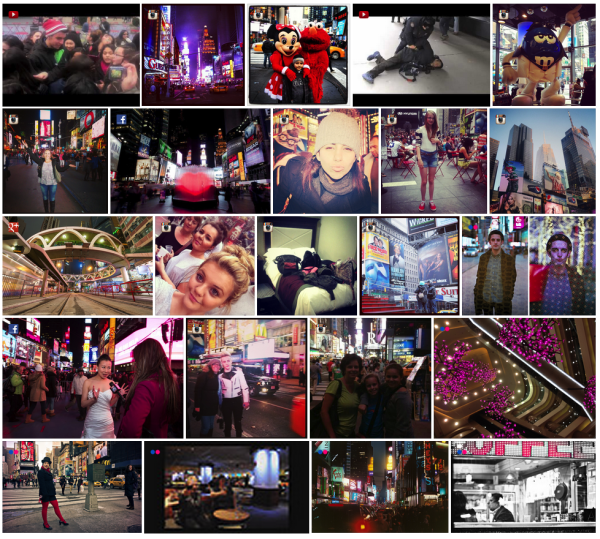
\includegraphics[height=5cm]{equal-size.png}
    \label{fig:a}
  }                
  \subfloat[\emph{LOVS}, Survey~A]{
    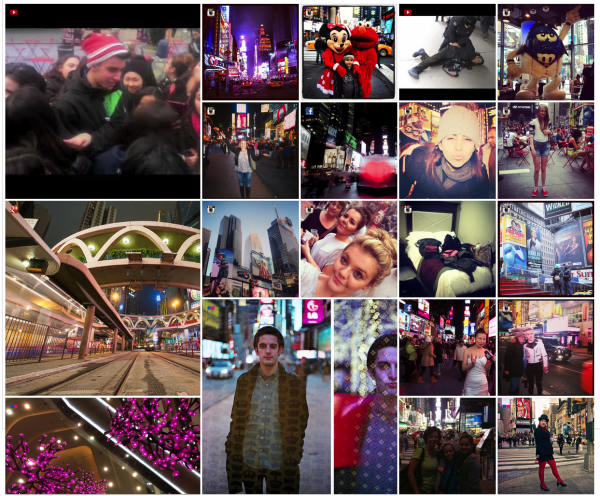
\includegraphics[height=5cm]{different-size.png}
    \label{fig:b}
  }
  \caption[Survey~A: Media galleries visualizing a~gathering at Times Square]{Survey~A: Media galleries visualizing a~gathering at Times Square, New York on February 8, 2013}
  \label{fig:media-gallery1}  
\end{figure}

\begin{figure}[!ht]
  \centering
  \subfloat[\emph{SOES}, Survey~B]{
    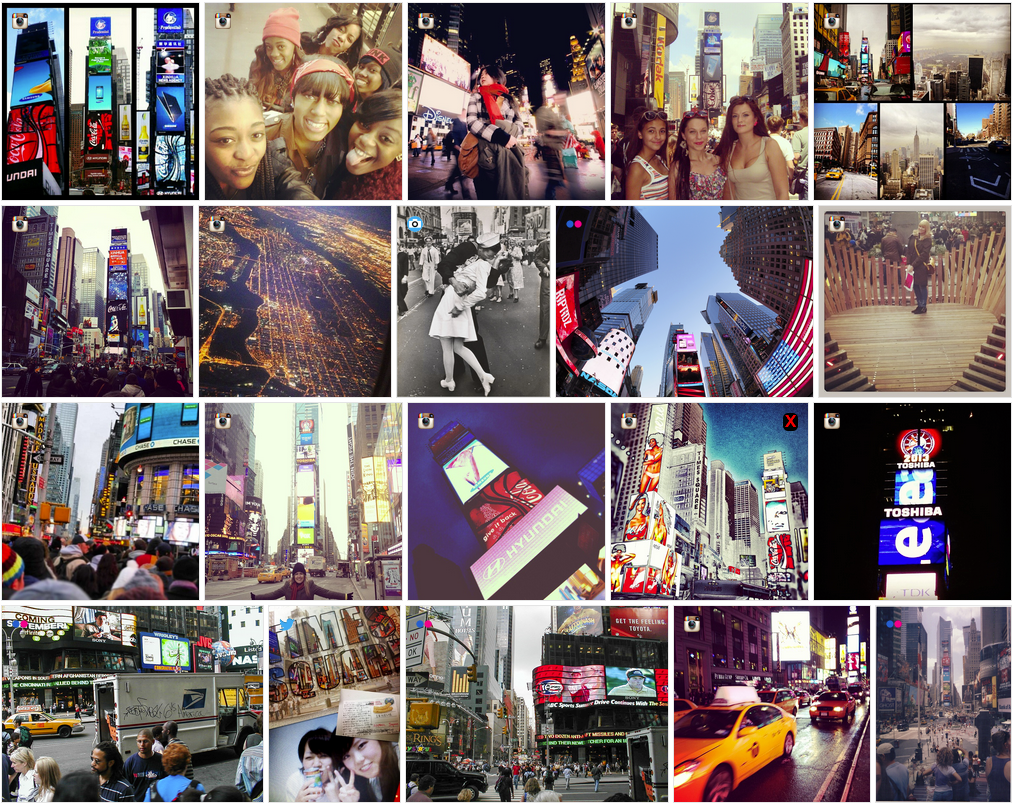
\includegraphics[height=5cm]{timessquare_2.png}
    \label{fig:c}
  }                
  \subfloat[\emph{LOVS}, Survey~B]{
    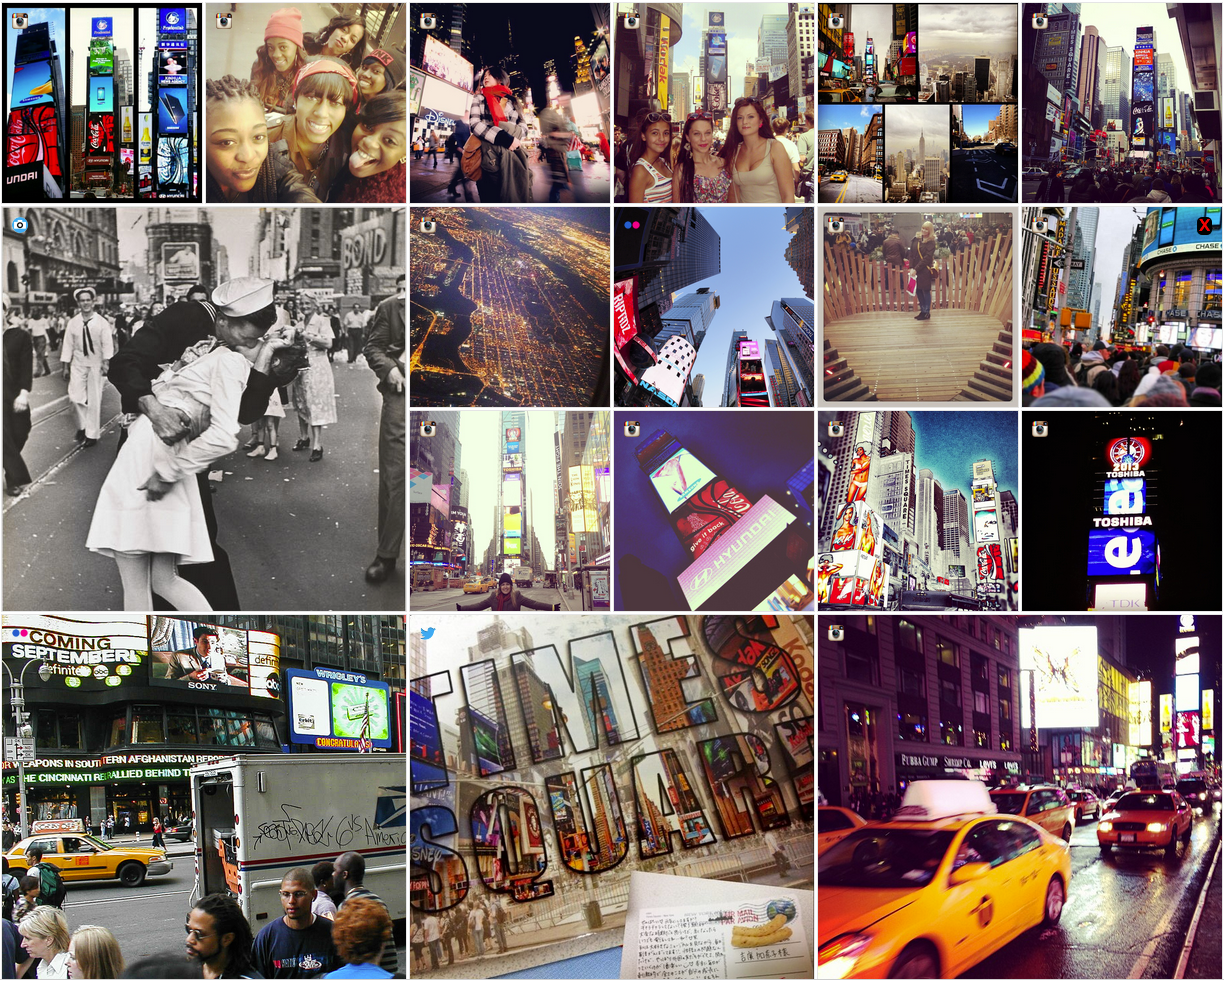
\includegraphics[height=5cm]{timessquare_1.png}
    \label{fig:d}
  }
  \caption[Survey~B: Media galleries visualizing a~gathering at Times Square]{Survey~B: Media galleries visualizing a~gathering at Times Square, New York on February 8, 2013}
  \label{fig:media-gallery2}  
\end{figure}

\paragraph{Loose Order, Varying Size (LOVS):}

Examples of a~media gallery style
that we call \emph{Loose Order, Varying Size (LOVS)}
can be seen in \autoref{fig:b} and \autoref{fig:d},
with the details explained in~\cite{chedeau2012facebook}.
The algorithm works by cropping all images to a~square aspect ratio,
which allows for organizing media items in a~way such
that one big square always
contains two horizontal blocks, each with two pairs of small squares.
The media gallery is then formed by iteratively filling
big or small squares until a~square is full
and then adding the square to the smallest column.
This media gallery style allows any media item to become big,
while still being loosely order-respecting and always hole-free.
Balancing the gallery is slightly harder,
as depending on the shape both small \emph{and} big
media items may be required.

\subsection{Discussion and Evaluation}
\label{sec:user-studies}

The main motivation for the \emph{Loose Order, Varying Size} style
is that certain media items can be featured more prominently
by making them big, while still loosely respecting the ranking-implied order.
Examples of to-be-featured media items can be videos,
media items with faces, media items available in High-Density quality,
or media items with interesting details~%
\cite{suh2003thumbnail}.
Users may want to decide what media items to feature,
albeit we aim for an automated solution.
Evaluating subjective data like \emph{the} correct presentation form
for a~set of media items is a~challenging task.
For different users and different media galleries,
there may be different optimal settings.
Again, we use the Mean Opinion Score (MOS,~\cite{itu1998mos})
for our evaluation, as previously motivated.

\paragraph{User Studies:}

We have conducted two types of surveys. 
Survey~A via multiple social networks, where we simply asked people to ``Like''
and/or comment on their favorite style of media gallery
and Survey~B that was distributed via email to a~company-internal ``miscellaneous'' mailing list,
where we asked people to rate media galleries via MOS, with optional comments. 
Survey~A and Survey~B used different media items in the media galleries,
as to have some measure in how far content has an impact.

\paragraph{Survey A---Via Social Networks:}

For Survey~A on the social networks Twitter, Facebook,
and \googleplus, we had overall 16~participants (7~female, 8~male, 1~unknown).
7~users liked \emph{SOES} more,
whereas 9~users liked \emph{LOVS} more.
Interestingly, no user commented on why they liked \emph{SOES} more.
Users who commented on why they liked \emph{LOVS} more mentioned
they liked the additional structure and tidiness,
the fact that some media items were bigger,
the fact that it was easier to identify individual media items,
and the fact that important media items were highlighted.

\paragraph{Survey B---Via Email:}

For Survey~B via email with MOS ratings,
we had 19~participants (6~female, 13~male).
The majority of users who liked \emph{LOVS} more
mentioned that the different sizes
gave the eye focal points and orientation,
whereas one user explicitly disliked this guidance.
Users liked the harmony and the structure.
Two users mentioned that small media items were proportionally too small.
Regarding \emph{SOES}, users reported they felt overloaded
and did not know where to start.
Some users said the layout was boring and that,
while they liked the outer framing,
they were confused by the irregular inner grid.
The MOS for \emph{SOES} was $2.39$ (variance $0.68$),
the MOS for \emph{LOVS} was $4.17$ (variance $0.47$).
The data of Survey~B is available.%
\footnote{\url{http://bit.ly/media-gallery-survey},
accessed July 15, 2013}
For privacy reasons, we have posted the media galleries
as non-public microposts on social networks,
which is why we are unable to share the data of Survey~A.

\subsection{Maintaining Provenance Information with Downloadable Media Galleries}

Media galleries consist of individual media items,
each with its specific pieces of provenance data
like creator, originating social network, \emph{etc.}
In the context of the application that we have developed
in the context of this thesis and
that will be described in full detail in \autoref{sec:socialmediaillustrator},
this provenance data is maintained in the form of HTML hyperlinks
back to the originating social networks.
However, when media galleries get downloaded in form of
one static image dump, this is no longer the case.
In consequence, we generate a~caption-like image legend
that gets added to each downloaded media gallery.
An example of a~media gallery with provenance data
generated in the context of the 2013 Taksim Gezi Park protests%
\footnote{\url{http://en.wikipedia.org/wiki/2013_Taksim_Gezi_Park_protests},
accessed July 15, 2013}
can be seen in \autoref{fig:occupygezidump}.

\begin{figure}[!ht]
  \centering
  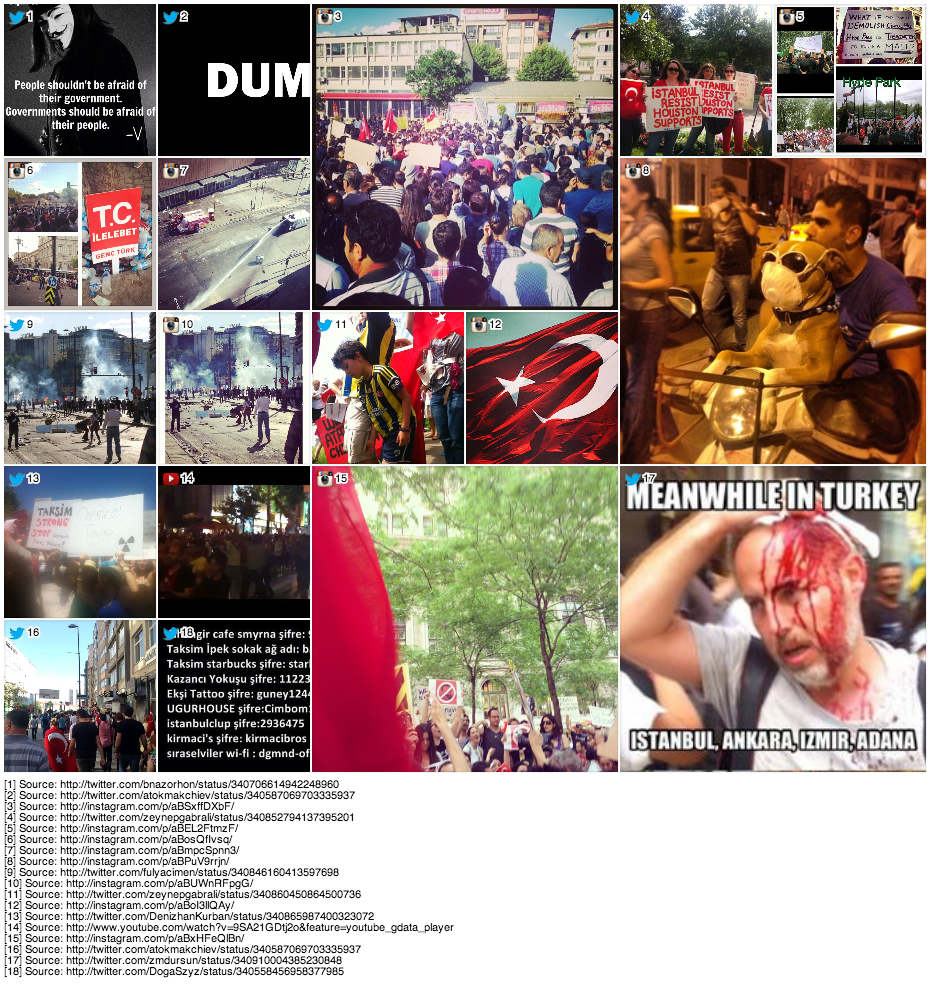
\includegraphics[width=1\columnwidth]{occupygezidump.png}
  \caption{Downloadable media gallery with provenance data}
  \label{fig:occupygezidump}
\end{figure}

\section{Interactive Media Galleries}
\label{sec:interactivemediagalleries}

\paragraph{Traditional slideshows:}

Up to now, we have presented different algorithms
to generate media galleries of different styles
and static media galleries, including a~way to preserve
provenance data when media galleries get downloaded as one image.
Such media galleries are useful in the context of static media,
such as newspapers or embedded in (online or offline) news articles.
A~first step towards more interactive media galleries are so-called slideshows.
An exemplary slideshow, courtesy of the BBC's Online division, can be seen in \autoref{fig:occupygezibbc}.

\begin{figure}[!ht]
  \centering
  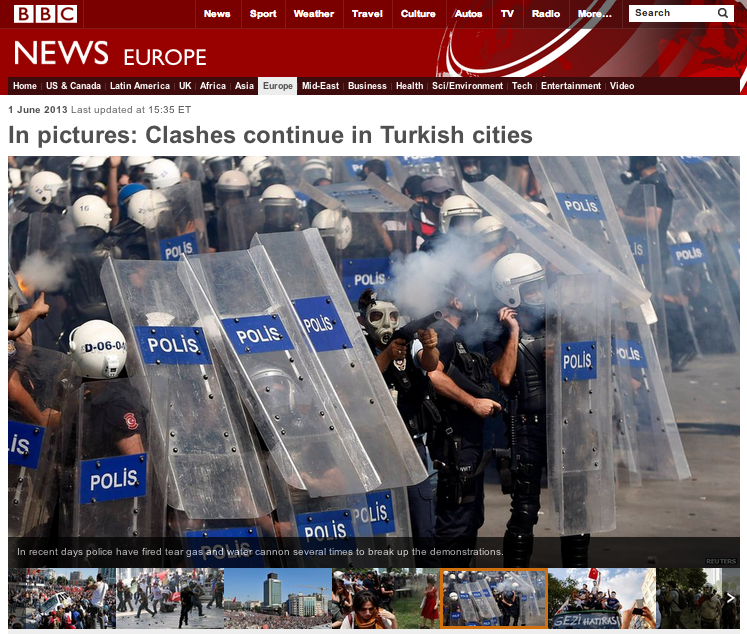
\includegraphics[width=0.8\columnwidth]{occupygezibbc.png}
  \caption[Media gallery in form of a~slideshow]{Media gallery in form of a~slideshow
  (Source and copyright: BBC Online \url{http://www.bbc.co.uk/news/world-europe-22740038}, accessed July 15, 2013)}
  \label{fig:occupygezibbc}
\end{figure}

\paragraph{Media gallery paradigm slideshows:}

We have opted to extend the traditional slideshow model
by adhering to the media gallery paradigm of our two preferred styles
Loose Order, Varying Size (\emph{LOVS}) and Strict Order, Equal Size (\emph{SOES}).
Given a~media gallery in either \emph{LOVS} or \emph{SOES} style,
each media item can be focused,
\emph{i.e.}, be put prominently in the foreground.
When a~media item is focused, it smoothly transitions
from its original location in the media gallery to the center,
while in parallel it is zoomed to double its size.
All other media items that are currently not focused are faded out
in a~black-and-white variant and blurred, in order to put the maximum emphasis
to the currently focused media item.
\autoref{fig:interactive-media-gallery} shows three steps of the described transitions and
\autoref{fig:occupygezi1} shows the final state after the transition.
A~screencast of the whole animation is available online at \url{https://vine.co/v/bT7eiwjE6DQ} (accessed July 15, 2013).

\begin{figure}[!ht]
  \centering
  \subfloat[Animation step 1]{
    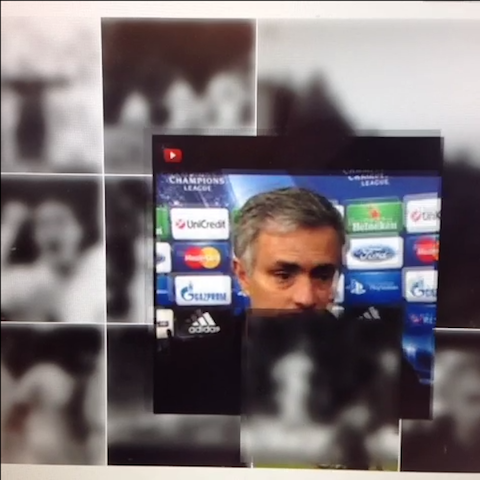
\includegraphics[height=4cm]{zoom1.png}
    \label{fig:zoom1}
  }                
  \subfloat[Animation step 2]{
    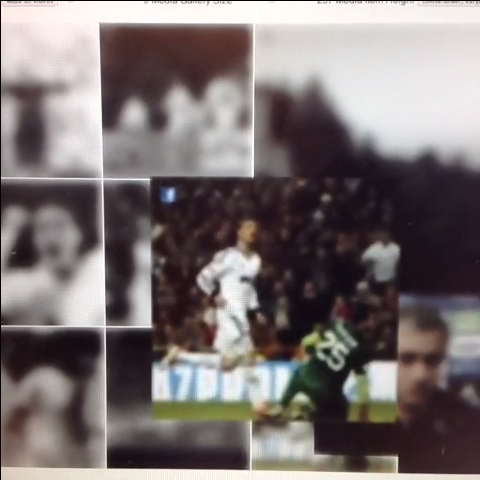
\includegraphics[height=4cm]{zoom2.png}
    \label{fig:zoom2}
  }
  \subfloat[Animation step 3]{
    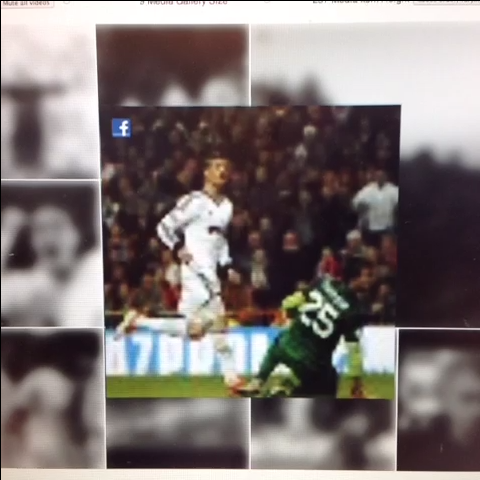
\includegraphics[height=4cm]{zoom3.png}
    \label{fig:zoom3}
  }  
  \caption[Three animation steps of interactive media gallery]{Three animation steps of interactive media gallery}
  \label{fig:interactive-media-gallery}  
\end{figure}

\paragraph{Audial media galleries and text-to-speech synthesis:}

With our media galleries, we go yet another step further
and add an audio component to the interactive slideshow.
As media items of type video typically already have an audio track,
it is thus straight-forward to play the video once it is focused
in the slideshow.
In contrast, photos do not have audible information associated with them.
We can, however, use the (potentially machine-translated,
see \autoref{sec:machine-translation}) textual information
of any of the media items in the particular media item's media cluster
(see \autoref{sec:photo-deduplication})
and via speech synthesis create an audial experience.
This follows the hypothesis that visually similar media items 
also share similar textual descriptions.
We use the set of extracted and disambiguated named entities
(see \autoref{sec:nlp-services}) combined with
the insights gained from part-of-speech tagging
(see \autoref{sec:part-of-speech-tagging})
to select the one textual description
from the entire set of textual descriptions in each cluster
that \textit{(i)} maximizes the number of named entities
and that \textit{(ii)} has the most diverse set of words
identified as nouns, verbs, and adjectives.
Following this heuristic, we effectively avoid choosing
a~textual description that only consists of a~list of tags,
as is often the case with, \emph{e.g.},
Instagram (see \autoref{sec:instagram}).
We convert the textual description of a~media item
to audial information with the help of a~text-to-speech system.
We use the eSpeak~\cite{duddington2012espeak} speech synthesizer
that was described earlier in \autoref{sec:from-debug-output-to-story}.

\begin{figure}[!ht]
  \centering
  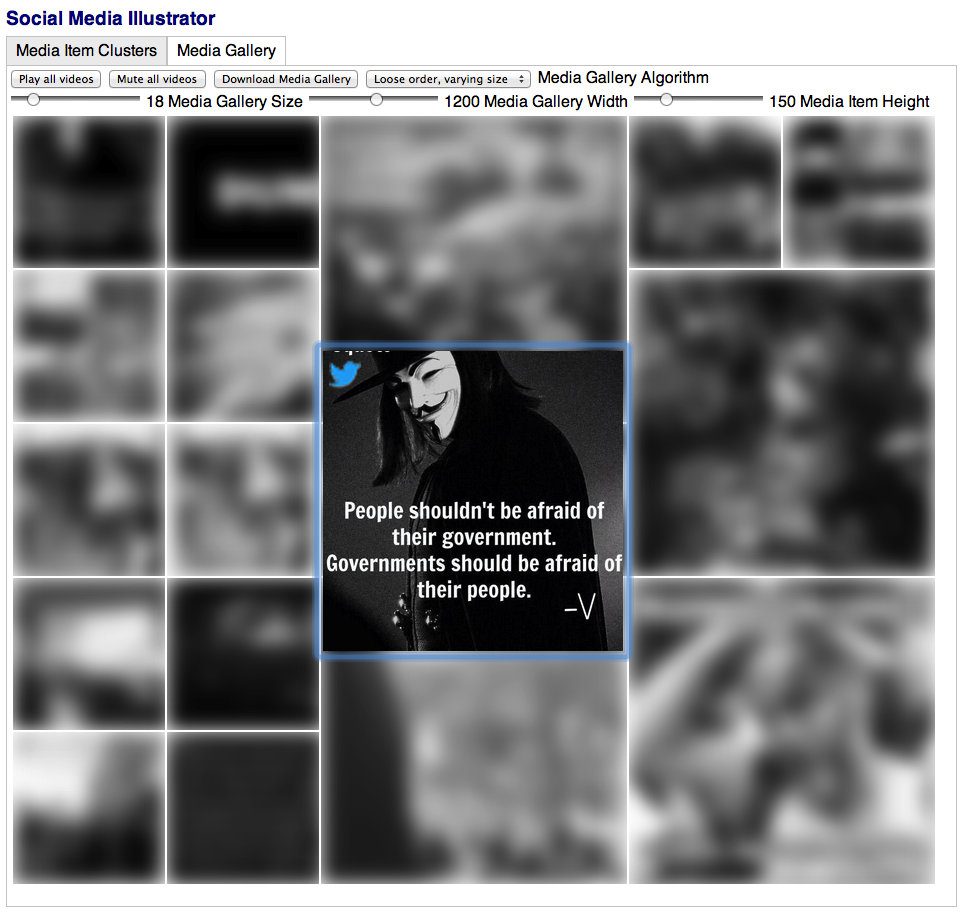
\includegraphics[width=1\columnwidth]{occupygezi1.png}
  \caption[Media gallery in interactive mode]{Media gallery in interactive mode, one media item centered and exclusively focused, all non-focused media items smoothly blurred and transitioned to a~black-and-white version}
  \label{fig:occupygezi1}
\end{figure}

\section{Social Media Illustrator}
\label{sec:socialmediaillustrator}

Media galleries that summarize given events
can be generated following the steps described in the previous chapters,
starting with micropost annotation (\autoref{cha:micropost-annotation}),
followed by event detection (\autoref{cha:eventdetection}),
continuing with media item extraction
(\autoref{cha:media-item-extraction}),
over to media item deduplication and clustering
(\autoref{cha:shot-boundary-detection} and  
\autoref{cha:media-item-deduplication}), 
media item ranking (\autoref{cha:media-item-ranking}) and
finally media item compilation (\autoref{cha:media-item-compilation}).
We have developed an application called \emph{Social Media Illustrator}
for the automated generation of
media galleries that visually and audially summarize events
based on media items like videos and photos from multiple social networks.
The application is publicly available at the URL 
\url{http://social-media-illustrator.herokuapp.com/} (accessed July 15, 2013).
\emph{Social Media Illustrator} implements all the abovementioned steps
and is a~start-to-end solution tailored to both
non-expert and expert users.
\autoref{fig:socialmediaillustratorscreenshot}
shows the start screen of the application.
The application has two tabs: \emph{``Media Item Clusters''} and \emph{``Media Gallery''}.

\begin{figure}[!ht]
  \centering
  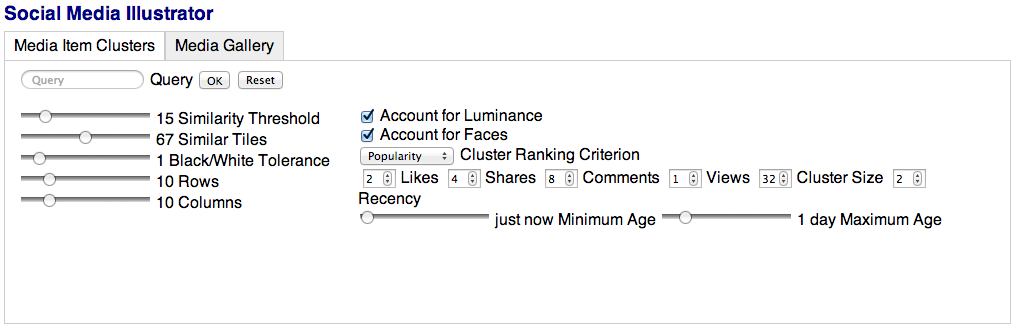
\includegraphics[width=1\columnwidth]{socialmediaillustrator.png}
  \caption{\emph{Social Media Illustrator} start screen}
  \label{fig:socialmediaillustratorscreenshot}
\end{figure}

\paragraph{Media Item Extraction:}

In a~first step, the user enters a~set of search terms
that are likely to reveal media items related to a~given event.
These search terms can be official event hashtags
(\emph{e.g.}, \texttt{\#VSFashionShow}
for the event described in \autoref{sec:vsfashionshow}),
but more commonly a~combination of names of the involved actors,
event names, event locations, or times~%
\cite{becker2010eventidentification,becker2012plannedevents}
like, for example, \emph{Stanley Cup 2013}.
Search results for each search term appear in the results panel
in the lower part of the graphical user interface
in form of a~so-called search bundle.
Search bundles are combined separate searches
that maintain mappings to the individual original search terms,
which can be enabled and disabled at will.
Undesired media items can be removed from the result bundle
by clicking a~red cross that appears
when hovering over the media item in question.
\autoref{fig:mediaitemextraction} shows \emph{Social Media Illustrator}
with extracted media items stemming from various social networks
for three search terms.

\begin{figure}[!ht]
  \centering
  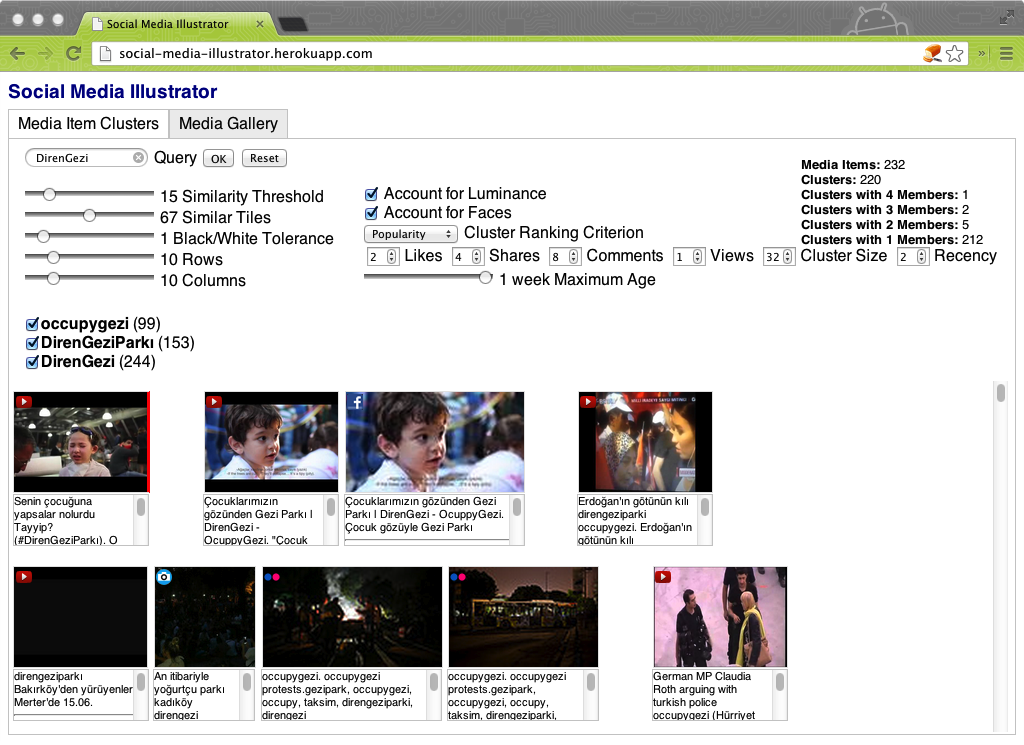
\includegraphics[width=1\columnwidth]{app1.png}
  \caption{Media item extraction with search bundles from three search terms}
  \label{fig:mediaitemextraction}
\end{figure}

\paragraph{Media Item Deduplication:}

Via the parameter settings on the left side, 
fine-grained control over the deduplicating
and matching algorithm is possible. 
The configurable options are described in \autoref{sec:media-item-deduplication-algorithm}.
Changes to any of the parameters are reflected in realtime
in the results panel below, which facilitates finding the optimal 
settings for a~given result set consisting of result bundles.
\autoref{fig:mediaitemdeduplication} shows the deduplication debug view (see \autoref{sec:media-item-deduplication-algorithm})
that is accessible by right-clicking two arbitrary media items.

\begin{figure}[!ht]
  \centering
  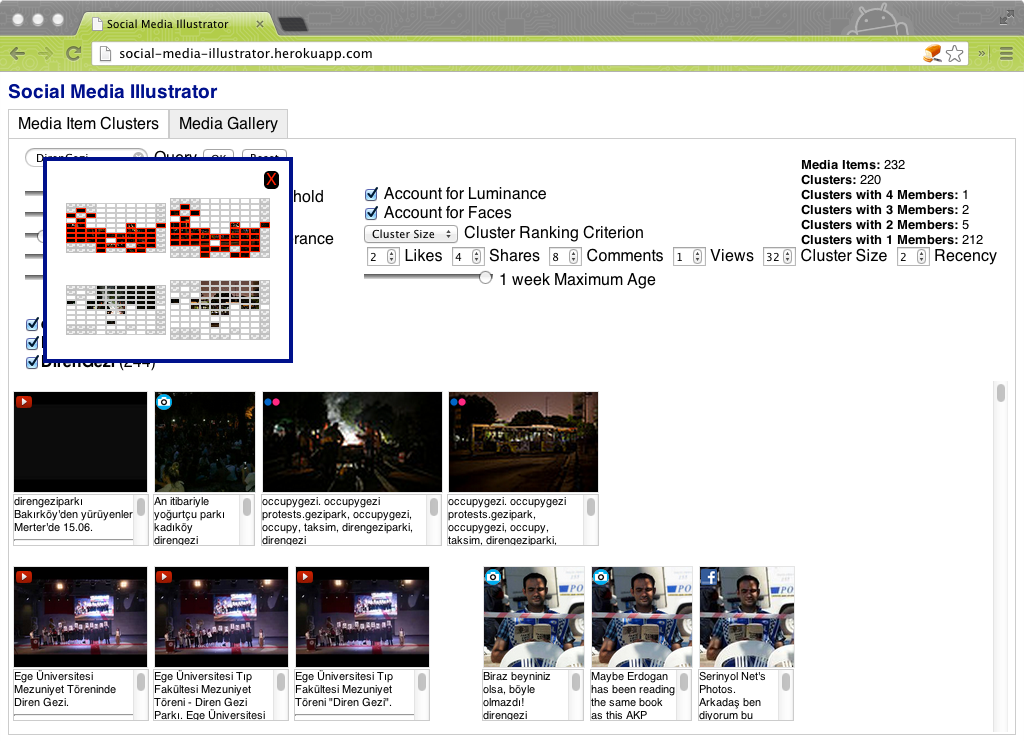
\includegraphics[width=1\columnwidth]{app2.png}
  \caption{Media item deduplication debug view}
  \label{fig:mediaitemdeduplication}
\end{figure}

\paragraph{Media Item Ranking:}

The parameter settings on the right side 
allow for interactively changing the ranking factors.
The user can select the main ranking criterion like recency or popularity, and modify the weight factors 
for the different ranking features in the ranking formula,
as detailed in \autoref{sec:introduction-of-a-ranking-formula}.
Again all changes are reflected in realtime.
A~slider control allows for selecting the maximum 
and minimum age of the considered media items 
in order to restrict the result set to a~given time period.
\autoref{fig:mediaitemranking} shows the select box
where the ranking formula can be selected.

\begin{figure}[!ht]
  \centering
  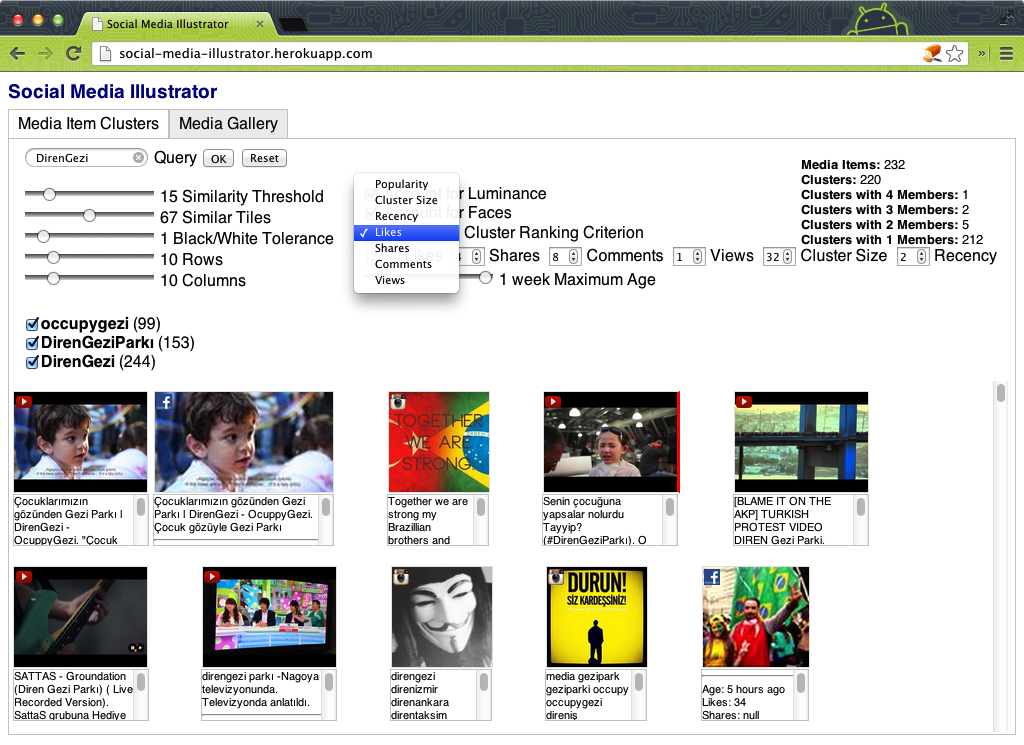
\includegraphics[width=1\columnwidth]{app3.png}
  \caption{Media item ranking with configurable ranking formula}
  \label{fig:mediaitemranking}
\end{figure}

\paragraph{Micropost Annotation:}

Once the user is happy with her selection and ranking of media items,
the next step is micropost annotation,
which---in contrast to the sequence suggested by the chapter order---%
only happens at this stage, based on only the final set of media items.
This is due to the fact that calling the external
named entity extraction and disambiguation services described in
\autoref{sec:nlp-services} is very expensive and time-consuming,
especially if an intermediate machine translation step is required.
This step happens transparently in the background,
while the media gallery is being compiled and is invisible to the user.

\paragraph{Media Item Compilation:}

The final step of media item compilation can be initiated
by clicking on the \emph{``Media Gallery''} tab.
A~configurable number of media items are compiled either in 
Loose Order, Varying Size (LOVS) style, or 
Strict Order, Equal Size (SOES), which was detailed in 
\autoref{sec:mediagallerystyles}.
The number of considered media items,
the width of the overall media gallery,
and the width of individual media items can be customized,
with the changes being reflected on-the-fly.
\autoref{fig:mediagallerycompilation1} shows a~media gallery
in the LOVS style.
By clicking on one of the media items,
the media gallery enters the interactive mode,
as can be seen in \autoref{fig:mediagallerycompilation2}.
Navigation from one media item to the next is possible via the arrow keys.

\begin{figure}[!ht]
  \centering
  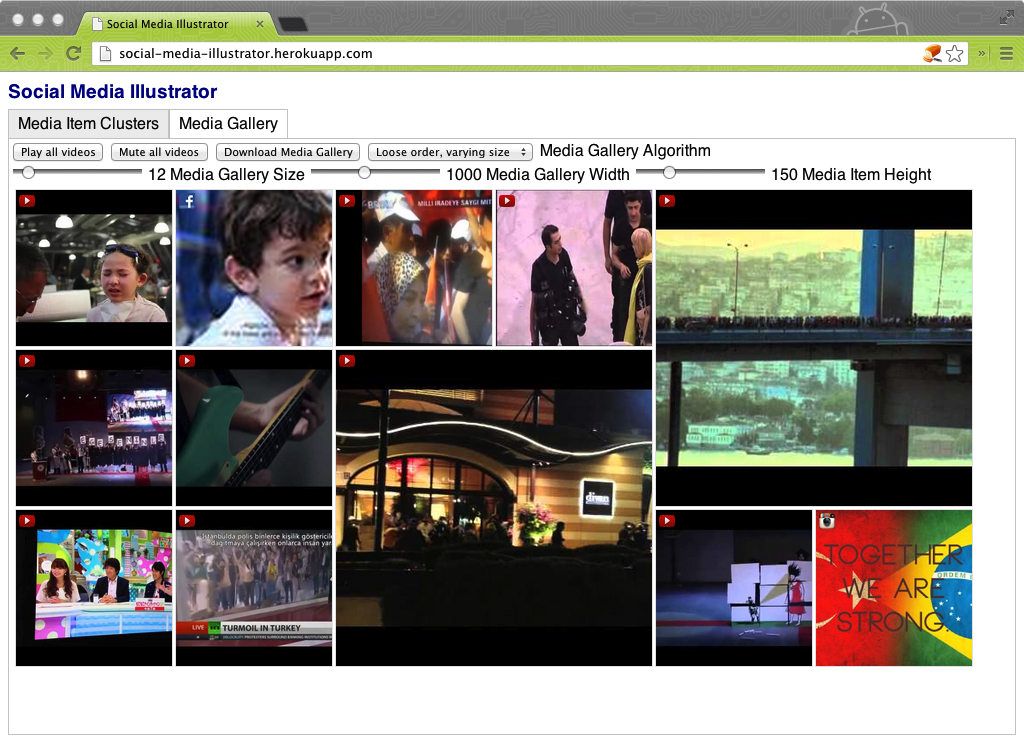
\includegraphics[width=1\columnwidth]{app4.png}
  \caption[Media gallery generation based on the Loose Order, Varying Sizes style]{Media gallery generation based on the Loose Order, Varying Sizes~(LOVS) style}
  \label{fig:mediagallerycompilation1}
\end{figure}

\begin{figure}[!ht]
  \centering
  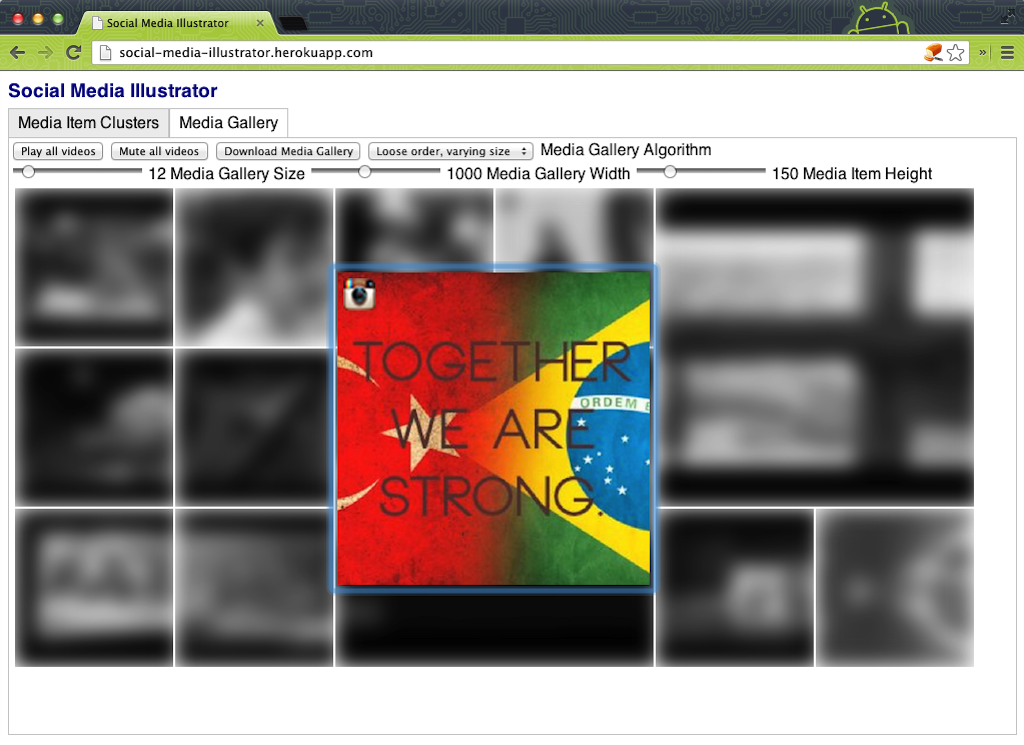
\includegraphics[width=1\columnwidth]{app5.png}
  \caption{Media gallery in interactive mode}
  \label{fig:mediagallerycompilation2}
\end{figure}

\section{Conclusions}

In this chapter, we have defined factors that determine and influence
media gallery aesthetics.
After an overview of related work and a~motivation,
we have examined different algorithms for the automated generation
of media galleries.
While some of the described algorithms do not fulfill our requirements
with regard to respecting the ranking-implied order,
two of them---namely \emph{LOVS} and \emph{SOES}---do fulfill them
and are in consequence considered.
We have created an application that auto-generates the
two media gallery styles \emph{SOES} and \emph{LOVS},
and evaluated users' perceived quality with two separate surveys. 
The trend is that users prefer \emph{LOVS}.
Future work will be on evaluating more media gallery styles
and advanced heuristics for media item cropping
tailored to social network media items.
As outlined earlier, such social media items
do not necessarily share the same properties as
common photos and videos.
Social media cropping algorithms need to respect 
the characteristics of social media
that were described in \autoref{sec:duplicate-content}.

We have learned that eyes need focal points
to spot the needles in the media gallery haystack.
Interactivity in form of visual \emph{eye candy}
as well as audial information are helpful factors
to create the impression of a~consistent \emph{event summarization}
that makes forget the fact that it was generated by combining potentially
many social network users' contributions.
Interactive media galleries help users process potentially
large amounts of data in an entertaining way.
Nevertheless---and besides all desired media gallery unity and consistency---%
we need to ensure that the individual social network user's contributions
are still traceable in the combined media gallery.
This is given for all use cases, offline and online.
Concluding, with our publicly accessible application \emph{Social Media Illustrator}
we have contributed a~valuable social media tool
that allows non-expert users to create event-summarizing media galleries at ease.

\section*{Chapter Notes}
This chapter is partly based on the following publication.
%\cite{steiner2013crop}.

\begin{itemize}
  \item \bibentry{steiner2013crop}.
\end{itemize}

\bibliographystyle{plainnat}
\clearpage
\bibliography{backmatter/references}
